\section{Background on binary rewriting}
\label{sec:background}

This section presents some background on binary rewriting and
discusses how security enforcement interacts with it. Our approach
relies on innovative binary rewriting
schemes~\cite{blind-kapil,blind-matt} incorporated into our binary
rewriting infrastructure called Secondwrite. Binary rewriters are
pieces of software that accept a binary executable program as input,
and produce an improved executable as output. The output executable
typically has the same functionality as the input, but is improved in
one or more metrics, such as run-time, energy use, memory use,
security or reliability.

\mypar{Advantages of binary rewriting} In recognition of its
potential, binary rewriting has seen much active research over the
last decade. The reason for great interest in this area is that binary
rewriting offers additional advantages over compiler-produced
optimized binaries:

\mybeginlist

\item \textbf{Ability to do inter-procedural optimization.} Although
  compilers in theory can do whole-program optimizations, the reality
  is that they do little if any. Many commercial compilers - even
  highly optimizing ones - limit themselves to separate compilation,
  where each file (and sometimes each function) is compiled in
  isolation. In contrast, binary rewriters have access to the complete
  application all at once, including libraries. This allows them to
  perform aggressive whole-program optimizations to exceed the
  performance of even optimized code. This ability can be useful for security schemes as well; in
    particular for those schemes that rely on whole-program information
    such as call graphs and inter-procedural properties to either work
    at all, or to optimize fully.

\item \textbf{Ability to do optimizations missed by the compiler.}
  Some binaries, especially legacy binaries or those compiled with
  inferior older compilers, often miss certain optimizations. Binary
  rewriters can perform these optimizations missed by the compiler
  while preserving the optimizations the compiler did 
  perform. This property may help the rewriter overcome some of the overheads
    of security enforcement by improvements in program run-time.

\item \textbf{Increased economic feasibility.} It is cheaper to
  implement a code transformation once for an instruction set in a
  binary rewriter, rather than repeatedly for each compiler for the
  instruction set. For example, the ARM instruction set has over 30
  compilers available for it, and the x86 has a similarly large number
  of compilers from different vendors and for different source
  languages. The high expense of repeated compiler implementation
  often cannot be supported by a small fraction of the demand. This
  implement-once property is useful for security schemes as well.

\item \textbf{Portable to any source language and any compiler.} A
  binary rewriter works for code produced from any source language by
  any compiler. This is a significant advantage when developing a
  security scheme such as the one presented in this paper. A scheme
  would not need to be ported to various compilers but would instead
  only need to be implemented once within a binary
  rewriter. Portability of rewriters aids security schemes implemented
  in them as well.

\item \textbf{Works for hand-coded assembly routines.} Code
  transformations cannot be applied by a compiler to hand-coded
  assembly routines, since they are never compiled. In contrast, a
  binary rewriter can transform such routines. Applying security in a
  binary rewriter has the advantage of working for hand-coded assembly
  versus compiler implementation of security, which does not.

\end{list}

%However, binary rewriters today have fallen far short of this desired
%vision. Binary rewriters remain relatively crude tools today, capable
%of no more than simple program transformations such as peephole
%optimization and code instrumentation. Complex transformations such
%as extensive whole-program optimizations, automatic parallelization
%and sophisticated security enforcement remain outside the
%capabilities of current rewriters.

% Padraig: I took the above paragraph out since the point here is to
% highlight all rewriters, not just ours.  Indeed it is not in the
% interests of this paper to make it seem like all the novelty is in
% our basic rewriter rather than your scheme.

\mypar{Architecture of Binary Rewriter} The binary rewriter developed
by our group and utilized for this research is named SecondWrite. Our
binary rewriter translates the input binary into the intermediate
representation (IR) of the LLVM compiler.  LLVM is a well-known
open-source compiler~\cite{llvm} developed at the University of
Illinois, and is now maintained by Apple Inc. LLVM IR is language- and
machine-independent. Our custom binary reader and de-compiler modules
read a binary and produce equivalent LLVM IR code.

Figure~\ref{swoverview} presents an overview of the SecondWrite
system. The SecondWrite system consists of a front-end module for
reading binary executables and generating an initial LLVM IR, an
internal pass module (not shown) for extracting more information about
the underlying program, optimizing passes to implement various
optimizations, and the LLVM code generator for producing the rewritten
binary.

\begin{figure}
\begin{center}
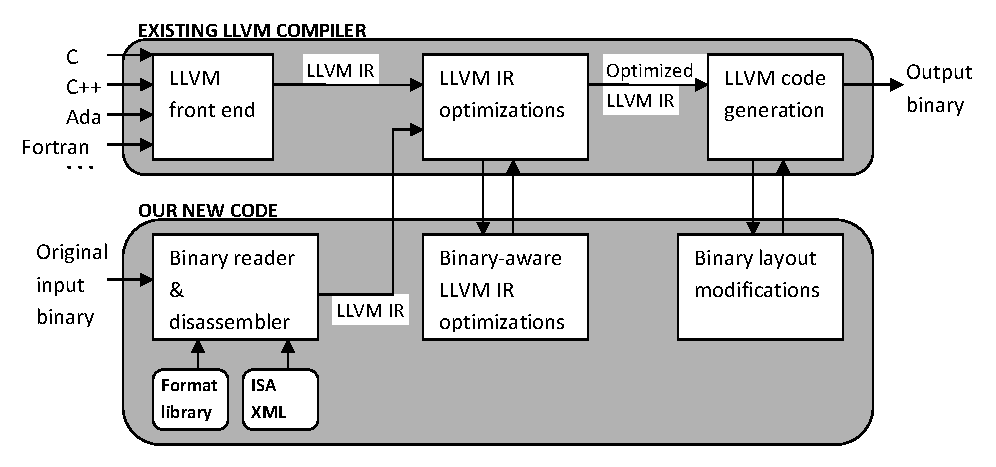
\includegraphics[scale=0.65]{images/flow.eps}
\end{center}
\renewcommand{\baselinestretch}{1}
\small\normalsize
\begin{quote}
\vspace{-0.2in}
\caption{SecondWrite system}
\label{swoverview}
\vspace{-0.5in}
\end{quote}
\end{figure}
\renewcommand{\baselinestretch}{2}

The front-end module consists of a disassembler and a custom binary
reader which processes the individual instructions and generates an
initial LLVM IR. This module reads the format of instructions from
Instruction Set Architecture (ISA) XML files for the ISA in question,
allowing for easy re-targeting of the rewriter to different
ISAs. Currently Secondwrite rewrites x86 and ARM binaries.

This initial representation is void of the desired IR features like
function prototypes, abstract stack and virtual registers. The
internal pass module analyzes this initial IR to obtain an improved IR
which has all the information and features mentioned
previously. Various existing and new LLVM optimization passes can be
applied on the above IR to obtain an optimized IR. Finally, the
optimized IR is passed to the existing LLVM code generator to obtain
the rewritten binary.

\mypar{Adding Security} Our approach to adding security to a binary is
to create numerous passes that work with the high-level IR. Working
with the high-level IR allows us to implement complex security
enhancements that would otherwise be difficult to add to a binary. We
discuss the various security methods we chose and implemented for this
paper in Section~\ref{sec:methods}. However, it is worth noting that
future research could easily focus on adding other security mechanisms
to the rewriter.

